% Supplementary material for the BlinkTwin manuscript. Build: latexmk -pdf supplement.tex
\documentclass[journal]{IEEEtran}
\usepackage[T1]{fontenc}
\usepackage{amsmath,amssymb}
\usepackage{graphicx}
\usepackage{booktabs}
\usepackage{array}
\usepackage{xcolor}
\usepackage{cite}
\usepackage{url}
\usepackage[hidelinks]{hyperref}
\graphicspath{{figures/}{../results/}{../docs/img/}}
\newcolumntype{L}[1]{>{\raggedright\arraybackslash}p{#1}}
\renewcommand{\thesection}{S\arabic{section}}
\renewcommand{\thetable}{S\arabic{table}}
\renewcommand{\thefigure}{S\arabic{figure}}
\renewcommand{\theequation}{S\arabic{equation}}

\begin{document}
\title{Supplementary Material for ``BlinkTwin: Questionnaire-Anchored Estimation and Forecasting of Subjective Sleepiness From Webcam and Reaction-Time Signals in a Web Browser''}
\author{Utsav~Poudel}
\markboth{Supplementary material}{Poudel: BlinkTwin}
\maketitle

\section{Workload model}
\label{sec:workload}
BlinkTwin also keeps an estimate of perceived workload $w(t)$ on the raw NASA-TLX scale (0--100)~\cite{hart1988development,hart2006nasa}. NASA-TLX rates a completed task, so treating a rating as a point observation of a momentary state is an approximation; the check-in therefore asks about the work block just finished. Workload reverts towards the demand $\mu_c$ of the current context $c$ as an Ornstein--Uhlenbeck process with time constant $\tau_w = 20$~min and stationary SD $\sigma_\infty = 18$. Over a step of $\Delta$ hours, with $\beta = e^{-60\Delta/\tau_w}$,
\begin{equation}
  w \leftarrow \mu_c + (w - \mu_c)\,\beta, \qquad P_w \leftarrow P_w\,\beta^2 + \sigma_\infty^2\,(1 - \beta^2).
\end{equation}
The demand of each context starts from a default $D_c$ (break 15, reading 40, focused work 65, meeting 50, other or unset 40) and is shrunk towards the person's own TLX ratings in that context, $\mu_c = (2D_c + \sum_i y_{c,i})/(2 + n_c)$. A TLX rating updates $w$ with noise SD $\sigma_T = 8$; the initial state is 40 with SD 20. The webcam is not used for workload. The defaults are assumptions, the same rating enters both the learned demand and the update, and the component has not been evaluated; it is therefore described as a feature of the application, not as a validated estimate of cognitive load~\cite{paas2003cognitive}.

\section{Three-Process Model constants}
\label{sec:tpm}
Table~\ref{tab:tpm} lists every constant of the prior with its source. All were checked by an independent reviewer against \cite{akerstedt2004predictions} and \cite{ingre2014validating}. The linear recovery rate below the breakpoint is the exponential's slope at the breakpoint, $\delta_s(H - B) = 0.80$ units~h$^{-1}$, following the construction in \cite{akerstedt2004predictions}. Sleep inertia uses the values of \cite{ingre2014validating}; the 2004 paper lists $W_{\mathrm{Decay}} = 0.65692$, which equals 1.51 divided by $\ln 10$ and is therefore probably a base-10 rate. Ingre et al.\ found that adding $W$ worsened the fit to airline data and refitted the KSS mapping to $a_K = 9.68$, $b_K = 0.46$~\cite{ingre2014validating}; the main paper tests that mapping on OpenNeuro ds004902.

\begin{table}[h]
  \centering
  \caption{Three-Process Model constants and sources}
  \label{tab:tpm}
  \footnotesize
  \begin{tabular}{@{}lll@{}}
    \toprule
    Constant & Value & Source \\
    \midrule
    Lower, upper asymptote of $S$ & 2.4, 14.3 & \cite{akerstedt2004predictions,ingre2014validating} \\
    Decay of $S$ awake & 0.0353 h$^{-1}$ & \cite{akerstedt2004predictions,ingre2014validating} \\
    Recovery of $S$ asleep & 0.381 h$^{-1}$ & \cite{akerstedt2004predictions,ingre2014validating} \\
    Breakpoint & 12.2 & \cite{akerstedt2008accounting,ingre2014validating} \\
    Circadian amplitude, acrophase & 2.5, 16.8 h & \cite{akerstedt2004predictions,ingre2014validating} \\
    Ultradian amplitude, mesor & 0.5, $-0.5$ & \cite{ingre2014validating} \\
    Ultradian dip & 13.8 h (and 01.8 h) & \cite{akerstedt2004predictions} \\
    Sleep inertia at waking, decay & $-5.72$, 1.51 h$^{-1}$ & \cite{ingre2014validating} \\
    KSS mapping & $10.6 - 0.6A$ & \cite{ingre2014validating} \\
    Habitual nights before history & 10 $\times$ 7.5 h & this work \\
    \bottomrule
  \end{tabular}
\end{table}

\section{DROZY: descriptive results}
\label{sec:drozy}
Fig.~\ref{fig:drozy} shows KSS across the three tests and its relation to PVT median reaction time and mean blink duration from the landmark pipeline. Fig.~\ref{fig:blink} shows the agreement of the landmark blink rates with EOG. In random-intercept mixed models, KSS rose by 2.22 points per 100~ms of median reaction time (95\% CI 1.07 to 3.37), 0.28 points per percentage point of PERCLOS (0.08 to 0.48) and 1.92 points per 100~ms of blink duration (0.71 to 3.14); these Wald intervals are anti-conservative with 14 clusters, the models do not separate within- from between-person effects, and the blink-rate model did not converge. They are reported for comparison with the earlier draft; the released model uses the within-person forward models of the main text instead. Per-subject slopes of KSS on reaction time, for the 9 subjects with three tests, ranged from 2.5 to 7.5 points per 100~ms, all positive; with three points per subject their spread cannot be separated from estimation noise.

\begin{figure}[h]
  \centering
  \includegraphics[width=\columnwidth]{fig_drozy.pdf}
  \caption{DROZY. KSS across the three tests, and KSS against PVT median reaction time and mean blink duration (landmark pipeline), one line per subject. Aggregate statistics only; no images.}
  \label{fig:drozy}
\end{figure}

\begin{figure}[h]
  \centering
  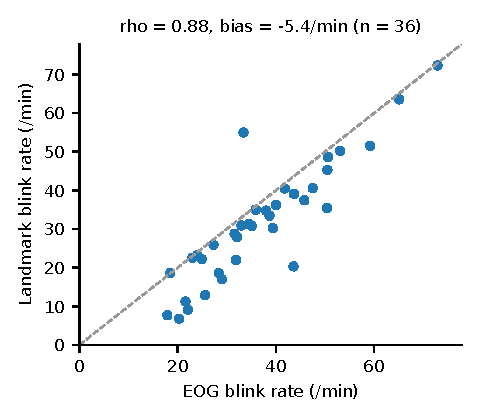
\includegraphics[width=0.75\columnwidth]{fig_drozy_blink_validation.pdf}
  \caption{Blink rate from the website's blink meter, run on DROZY landmarks, against blink rate from the vertical EOG, one point per test ($n = 36$).}
  \label{fig:blink}
\end{figure}

\section{OpenNeuro ds004902: details}
\label{sec:openneuro}
Fig.~\ref{fig:openneuro} shows the KSS and PVT median reaction time in the two sessions and the coupling of the reaction-time change with the SSS change. For the offset analysis, the KSS time was the eyes-open EEG time of each session; the normal-sleep session assumed a 7.5-h night ending at 07:00 and the deprivation session assumed waking at 07:00 on the previous day. The sleep-diary analysis used the diary's bedtime and get-up time for the normal-sleep night (28 people with KSS in both sessions and a diary between 3 and 13~h), and the diary's get-up time as the previous wake time for the deprivation session. The shrinkage factor for one check-in was the Kalman gain $\sigma_d^2/(\sigma_d^2 + \sigma_K^2) = 0.72$; in the persistence analysis it was estimated from the data as 0.77.

\begin{figure}[h]
  \centering
  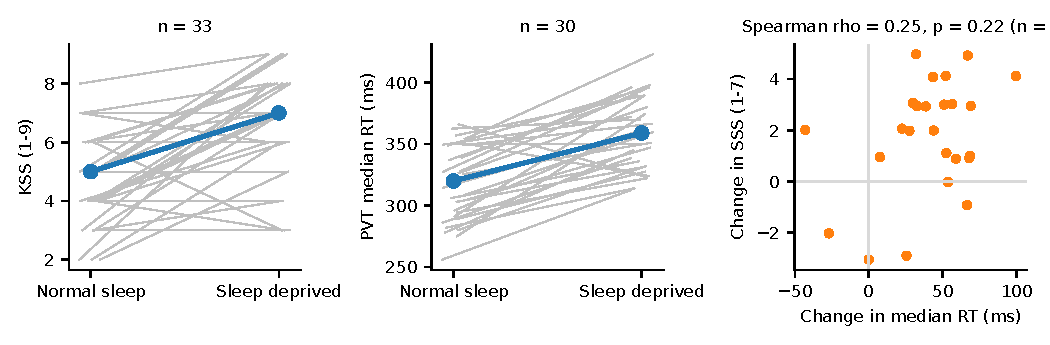
\includegraphics[width=\columnwidth]{fig_openneuro.pdf}
  \caption{OpenNeuro ds004902. Left and middle: KSS and PVT median reaction time after normal sleep and after sleep deprivation (grey: individuals; blue: medians). Right: change in median reaction time against change in SSS for the 25 people with both.}
  \label{fig:openneuro}
\end{figure}


\section{Simulation details}
\label{sec:simdetails}
\paragraph*{Virtual people} Person-level parameters: offset $o \sim \mathcal{N}(0, 0.84)$; circadian phase shift $\mathcal{N}(0, 1)$~h; time-on-task effect $\mathcal{N}(0.4, 0.2)$ KSS~h$^{-1}$, truncated at 0; slow fluctuation of sleepiness (Ornstein--Uhlenbeck, SD 0.5, time constant 1.5~h); rating noise SD 0.7, rounded and clipped to 1--9. Each passive feature follows $a_i + b_i (s^* - 3)$ with $a_i \sim \mathcal{N}(a, \sigma_\alpha)$ and $b_i \sim \mathcal{N}(b, \cdot)$ truncated at 0, using the DROZY values of Table~II of the main paper (reaction-time slope SD 8~ms, blink-duration slope SD 7~ms, PERCLOS slope SD 0.3\%). Webcam baselines drift (Ornstein--Uhlenbeck, SD 30~ms for blink duration and 1.8\% for PERCLOS, time constant 4~h) and per-minute noise is AR(1) with $\rho = 0.02$ (blink duration) and 0.32 (PERCLOS). Truncations: median reaction time $\geq 180$~ms; blink duration $\geq 60$~ms; PERCLOS in 0--60\%; blink rate $\mathcal{N}(18, 6)$ per minute, rounded, with blink duration missing below 3 blinks; face coverage fixed at 0.9.

\paragraph*{Scenarios} \emph{Misreport}: circadian phase SD 2~h and actual sleep differing from the reported 7.5~h with SD 1.5~h. \emph{Nonlinear}: signals respond with 0.6 of the slope up to KSS~6 and an added quadratic term above it; Student-$t_3$ noise. \emph{Rating bias}: a personal bias SD 0.8 added to every rating and rating noise SD 1.0. \emph{Autocorrelated webcam}: per-minute noise AR(1) with $\rho = 0.7$ and larger baseline drift. \emph{Trait}: homeostatic decay multiplied by $e^{\mathcal{N}(0, 0.3)}$ and circadian amplitude by $e^{\mathcal{N}(0, 0.2)}$ per person. \emph{Debt}: five previous nights of 5~h, of which the model is told only the last. \emph{Workday}: 16~h awake (07:30--23:00), check-ins 08:30--21:30, forecasts 09:00--22:00. \emph{Dissociation}: ratings equal the truth up to KSS~5 and include only half of any further rise.

\begin{table*}[t]
  \centering
  \caption{MAE of latent KSS at three check-ins by scenario, and the paired difference BlinkTwin minus check-ins only (95\% CI; share of people for whom BlinkTwin was better)}
  \label{tab:scenarios}
  \footnotesize
  \setlength{\tabcolsep}{5pt}
  \begin{tabular}{@{}lccccccc@{}}
    \toprule
    Scenario & Prior & Check-ins & No anchors & BlinkTwin & Oracle & Difference (95\% CI) & Better \\
    \midrule
    Matched & 0.819 & 0.659 & 1.741 & 0.629 & 0.586 & $-0.030$ ($-0.042$, $-0.016$) & 64\% \\
    Misreport & 0.924 & 0.763 & 1.735 & 0.711 & 0.660 & $-0.052$ ($-0.065$, $-0.039$) & 66\% \\
    Nonlinear & 0.837 & 0.671 & 1.754 & 0.633 & 0.615 & $-0.037$ ($-0.051$, $-0.024$) & 63\% \\
    Rating bias & 0.819 & 0.918 & 1.742 & 0.863 & 0.691 & $-0.055$ ($-0.071$, $-0.039$) & 68\% \\
    Autocorrelated & 0.819 & 0.659 & 2.026 & 0.646 & 0.657 & $-0.013$ ($-0.027$, $+0.001$) & 53\% \\
    Trait & 0.969 & 0.697 & 1.728 & 0.656 & 0.606 & $-0.042$ ($-0.055$, $-0.029$) & 66\% \\
    Debt & 0.858 & 0.633 & 1.768 & 0.598 & 0.557 & $-0.035$ ($-0.047$, $-0.023$) & 65\% \\
    Workday & 0.832 & 0.682 & 1.732 & 0.661 & 0.640 & $-0.021$ ($-0.036$, $-0.007$) & 56\% \\
    Dissociation & 0.819 & 0.665 & 1.742 & 0.636 & 0.585 & $-0.029$ ($-0.042$, $-0.015$) & 62\% \\
    \bottomrule
  \end{tabular}
\end{table*}

\begin{table}[h]
  \centering
  \caption{Sensitivity of the matched scenario at three check-ins to the assumed filter settings (default in bold)}
  \label{tab:sensitivity}
  \footnotesize
  \setlength{\tabcolsep}{3pt}
  \begin{tabular}{@{}llcccc@{}}
    \toprule
    Setting & Value & \multicolumn{2}{c}{MAE} & \multicolumn{2}{c}{Coverage} \\
    \cmidrule(lr){3-4}\cmidrule(l){5-6}
    & & Check-ins & BlinkTwin & Check-ins & BlinkTwin \\
    \midrule
    Offset prior SD $\sigma_d$ & 0.84 & 0.647 & 0.614 & 0.90 & 0.90 \\
     & \textbf{1.2} & 0.659 & 0.629 & 0.91 & 0.90 \\
     & 1.6 & 0.671 & 0.647 & 0.91 & 0.90 \\
    Offset drift $\sqrt{q_d}$ & 0.15 & 0.629 & 0.615 & 0.82 & 0.81 \\
     & \textbf{0.3} & 0.659 & 0.629 & 0.91 & 0.90 \\
     & 0.6 & 0.720 & 0.708 & 0.98 & 0.96 \\
    Time on task $\gamma$ & 0 & 0.653 & 0.620 & 0.91 & 0.91 \\
     & \textbf{0.4} & 0.659 & 0.629 & 0.91 & 0.90 \\
     & 0.8 & 0.700 & 0.669 & 0.88 & 0.88 \\
    Rating noise $\sigma_K$ & 0.5 & 0.707 & 0.668 & 0.82 & 0.82 \\
     & \textbf{0.75} & 0.659 & 0.629 & 0.91 & 0.90 \\
     & 1.0 & 0.630 & 0.618 & 0.95 & 0.94 \\
    Anchor drift ($\times$) & 0.5 & 0.659 & 0.657 & 0.91 & 0.87 \\
     & \textbf{1} & 0.659 & 0.629 & 0.91 & 0.90 \\
     & 2 & 0.659 & 0.635 & 0.91 & 0.90 \\
    Slope spread ($\times$) & 0 & 0.659 & 0.633 & 0.91 & 0.90 \\
     & \textbf{1} & 0.659 & 0.629 & 0.91 & 0.90 \\
     & 2 & 0.659 & 0.628 & 0.91 & 0.90 \\
    \bottomrule
  \end{tabular}
\end{table}

\begin{figure}[h]
  \centering
  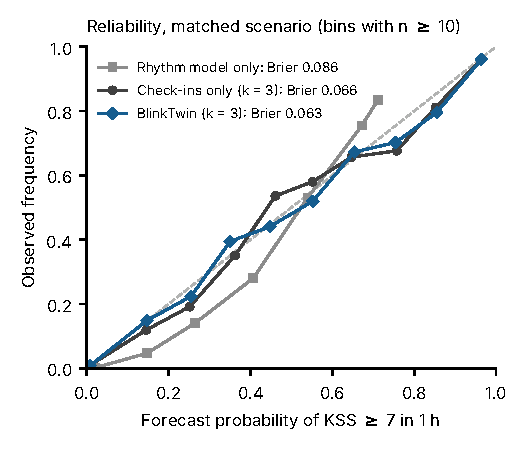
\includegraphics[width=\columnwidth]{fig_sim_reliability.pdf}
  \caption{Reliability of the one-hour forecast of latent KSS $\geq 7$ in the matched scenario at three check-ins (10 equal-width bins; 5400 forecasts from 300 virtual people). Points on the diagonal are perfectly calibrated.}
  \label{fig:reliability}
\end{figure}


\bibliographystyle{IEEEtran}
\bibliography{refs}
\end{document}
